
\begin{table}[t]
\centering
\caption {Notations}
\scalebox{0.7}{
 \begin{tabular}{l|l}  \toprule
 \multicolumn{1}{c}{\textbf{Symbol} } &  \multicolumn{1}{c}{\textbf{Explanations}}\\\midrule
\textbf{Boldface}& \text{- represents encrypted data}\\
$\tilde{}$ & \text{- represents one-hot-coding}  \\  $\hat{}$ & - represents a differentially private output  \\ $A$ &- an attribute  \\ $s_A$ &- size of domain of attribute $A$
\\$dom(A)=\{v_1,\ldots,v_{s_A}\}$ & - domain of attribute $A$\\ $ct_{A,i}$  &- \# \text{records with value $v_i$ for attribute} A\\ $m$   &- \text{\# number of data onwers}\\ $\boldsymbol{\tilde{\mathcal{D}}}$  &- \text{encrypted database with records in}\\&\text{  per-attribute one-hot-coding } \\ %$\mathcal{A}=\{\mathcal{A}_1,...\mathcal{A}_l\}$   &- \text{set of attributes in the schema of $\boldsymbol{\tilde{\mathcal{D}}}$}\\
$x \times y \text{ table } \mathbf{T}$   &- \text{an encrypted table  with $x$ records in}\\&\text{ one-hot-coding and $y$ columns one for}\\&\text{ each attribute; serves as one of the }\\&\text{ inputs to a transformation primitive}\\ $\mathbf{B}$&- \text{a vector of length $m$ such that each entry}\\&\text{ $\textbf{B}[i]$ represents whether record $r_i, i \in [m]$}\\& \text{is relevant to the program at hand} \\ $V$ & -\text{ represents a vector}\\$c$ &- \text{represents a scalar}\\$\mathcal{P}$ & - \text{represents a set}\\
 \bottomrule
 \end{tabular}}
 \label{Notations}
\end{table}

\begin{figure}[t]
	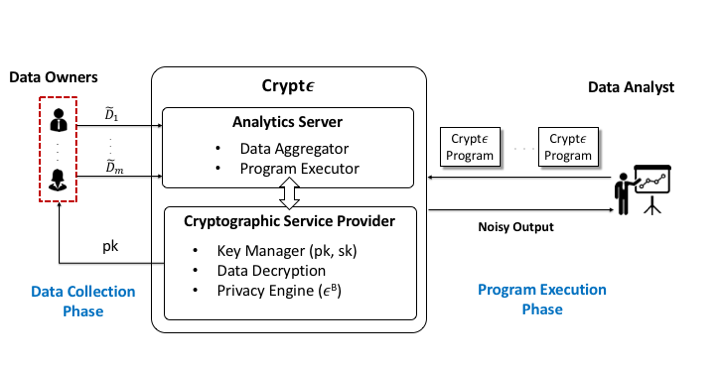
\includegraphics[width=\columnwidth]{diag.png}
	\caption{\label{fig:system} Crypt$\epsilon$ System}% Setting: The  \textsf{AS} runs the Crypt$\epsilon$ programs. The \textsf{CSP} manages the cryptographic primitves. } 
\end{figure}


\section{\system Overview}\label{sec:overview}
In this section, we describe \system's architecture (Sec~\ref{sec:arch}), the different modules in the system (Sec~\ref{sec:modules}), and the trust assumptions made by our system (Sec~\ref{sec:trust}). We end with a brief discussion justifying the design of \system (Sec~\ref{sec:discuss-arch}). 

\subsection{System Architecture}\label{sec:arch}
\system's architecture is illustrated in Figure~\ref{fig:system}. A set of \textit{data owners} ${DO_i, i\in [m]}$ have private data records ${D_i, i \in [m]}$. \system permits analysts to author and execute programs $P$ that satisfy differential privacy under the \cdp model without storing or computing on the private data records in the clear. \system achieves this by aggregating encrypted private records at the \textit{analytics server} \textsf{AS}. Keys needed for encrypting private records and decrypting answers are managed by the \textit{crypto servide provider} \textsf{CSP} so that the data owner need not participate in the differentially private computation.    

\system operates in three phases: 
 \squishlist
 \item \textbf{Setup Phase}: In the first phase, data owners initializes a \textsf{CSP} with a privacy budget $\epsilon^B$, which is stored in the \textsf{CSP}'s \textit{privacy manager} module. Next, the  \textsf{CSP}'s \textit{key manager} module generates the key pairs for labHE $(sk,pk)$, publishes $pk$ to the data owners and stores $sk$. 
 \item \textbf{Data Collection Phase}: In the next phase, each data owners encodes and encrypts their records using the \textit{data encoder} and \textit{data encryption} modules. The data owners send the encrypted data records to the \textsf{AS}. The data owners are relieved of all other duties and can go completely off-line. The \textit{aggregator} module of the \textsf{AS} then aggregates these encrypted records into a single encrypted database $\boldsymbol{\tilde{\mathcal{D}}}$. 
 \item \textbf{Program Execution Phase}: In this phase, the \textsf{AS} executes a \system program provided by the analyst. \system programs (which are described in more detail in Sections~\ref{sec:primitives} and \ref{sec:implementation}) access the sensitive data using a restricted set of data transformation, that filter, count or group the sensitive data, and measurement primitives, which are differentially private operations to release noisy answers. A majority of the data transformation operations are executed wholly at the \textsf{AS}. However, every measurement operator requires an interaction with the \textsf{CSP} as it requires (a) decryption of the answer, and (b) a check that the the privacy budget is not exceeded. These two functionalities are achieved by the \textit{decryption} and \textit{privacy engine} modules of the \textsf{CSP}. 
 \squishend
 The \emph{Setup} and \emph{Data Collection} phases occur just once at the very beginning, every subsequent program  is handled via the corresponding  \emph{Program Execution} phase. We next detail the roles of the different modules in the data owners, the analytics server and the crypto service provider.  
 
\subsection{\system Modules}\label{sec:modules}

\stitle{Cryptographic Service Provider (\textsf{CSP})}\\
(1)\textbf{ Key Manager }- The foremost duty of the \textsf{CSP} is to initialize the encryption scheme of Crypt$\epsilon$. This task is handled by the \textit{Key Manager} module which generates the key pair $(sk,pk)$ for the \textsf{labHE} scheme. It stores the secret key, $sk$ with itself and releases the public key, $pk$. Note that since the \textsf{CSP} has exclusive access to the secret key $sk$, it is the only entity capable of decryption in Crypt$\epsilon$.\\
(2)\textbf{ Data Decryption }- The \textsf{CSP} being the only entity capable of decryption,  any measurement of the data (even noisy) has to involve the \textsf{CSP}. The \textit{Data Decryption} module is tasked with handling all such interactions with the \textsf{AS}. \\
(3)\textbf{ Privacy Engine }- Crypt$\epsilon$ starts of with a total privacy budget of $\epsilon^B$ which is unanimously agreed upon by all the data owners. Note that the mechanism of deciding $\epsilon^B$ should be piloted by social prerogatives \cite{e1,e2} 
and is currently outside the scope of Crypt$\epsilon$. For executing any program, the \textsf{AS} has to interact with the \textsf{CSP} at least once (for decrypting the noisy answer) thereby giving the \textsf{CSP} the opportunity to monitor the \textsf{AS}'s actions in terms of privacy budget expenditure. The \textit{Privacy Engine} module hence maintains a public ledger that records the privacy budget spent in executing each program. Once the privacy cost incurred reaches 
$\epsilon^B$, the \textsf{CSP} refuses to decrypt any further answers thereby ensuring that the privacy budget is not exceeded.  The ledger is completely public allowing any data owner to verify it as and when desired.\\
\stitle{Data Owners (\textsf{DO})}\\
(1)\textbf{ Data Encoder} -  Each data owner $\textsf{DO}_i, i \in [m]$ has a private data record $D_i$ of the form $\langle A_1,...A_l\rangle$ where ${A}_j$ is an attribute. At the very outset, every data owner  $\textsf{DO}_i$ represents his/her private record $D_i$ in its respective per attribute one-hot-coding format. The one-hot-coding is a way of representation for categorical attributes and is illustrated by the following example. 
If the database schema in \system is given by  $\langle Age,Gender\rangle$ then corresponding one-hot-coding representation for a data owner $DO_i, i \in [m]$ with the record $\langle 30, Male\rangle$, is given by $\tilde{D_i}=\langle[\underbrace{0,\ldots,0}_{29},1,\underbrace{0,\ldots,0}_{70}],[1,0]\rangle$. \\
(2)\textbf{ Data Encryption} - The \textit{Data Encryption} module stores the public key $pk$ of the labHE scheme used in Crypt$\epsilon$ which is announced by the CSP. This key is used for an element-wise encryption of the data owner's  record of per attribute one-hot-codings. In our aforementioned example, we get $\mathbf{\tilde{D}}=\langle[\underbrace{labEnc_{pk}(0),\ldots}_{29},labEnc_{pk}(1),\\\underbrace{\ldots,labEnc_{pk}(0)}_{70}],
[labEnc_{pk}(1),labEnc_{pk}(0)]\rangle$. Finally the data owner sends this encrypted record to the \textsf{AS} via a secure channel. This is the only interaction that a data owner ever participates in, all the program executions are carried out by the \textsf{AS} and the \textsf{CSP} with the data owners being completely off line.\\
\stitle{Analytics Server (\textsf{AS)}}\\
(1)\textbf{  Aggregator} - The \textit{Aggregator} collects the encrypted records $\mathbf{\tilde{D_i}}$ from each of the data owners $\textsf{DO}_i$ and collates them into a single encrypted database $\boldsymbol{\tilde{\mathcal{D}}}$. %Note that in contrast, the server in the \textsf{CDP} model, being trusted, stores the data in the clear whereas in the \textsf{LDP} model the untrusted server stores appropriately randomized (noisy) data.   
\\(2)\textbf{ Program Executor }- The \textit{Program Executor} is the most important module of the \textsf{AS} and is tasked with the execution of Crypt$\epsilon$ programs. It takes as input a Crypt$\epsilon$ program from an external data analyst, alongside the appropriate privacy parameter $\epsilon$ and publishes the differentially private output computed with the assistance of the \textsf{CSP}. Crypt$\epsilon$ supports a set of 9 primitives and a Crypt$\epsilon$ program is an execution plan expressed as a sequence of these primitives. The primitives can be broadly classified into two types- transformation primitives and measurement primitives. Transformation primitives allow certain modifications on the encrypted data and are performed almost entirely by the \textsf{AS}. The measurement primitives on the other hand reveal some noisy measurement of the data and requires interaction with the \textsf{CSP}. \system supports two types of measurement primitives that implement two of the most popular differentially private mechanisms, Laplace mechanism \cite{Dork} and Noisy-Max \cite{Dork}. A typical Crypt$\epsilon$ program execution consists of  a series of transformation on the encrypted data followed by a measurement primitive and arbitrary post-processing. \\
 \textit{Noise Addition in \system} - For the Laplace mechanism, both the \textsf{AS} and the \textsf{CSP} add two separate instances of the random noise to the program output. This is necessary because had only one of them added the noise, then after the release of the clear text output, that party can simply subtract out the noise to reveal the true private answer. An alternative way can be both \AS and \CSP jointly computing a single instance of the noise using a secure computation protocol (see Appendix D.1). However, we do not implement it in the current version of \system as the two-fold noise addition is more efficient. For the Noisy-Max primitive, we provide an efficient secure computation protocol where only a single instance of noise by either party suffices. 
Since in Crypt$\epsilon$ the point of noise addition is just at the two servers, unlike at every individual in \textsf{LDP}, we achieve constant error bounds which is of the same order as that of \textsf{CDP} (see section \ref{exp:results}). 
 

\am{Not sure where this one goes ... move to discussion?}
Figure 1 shows the diagrammatic representation of \system. A comparative analysis of \system, \textsf{CDP} and \textsf{LDP} is presented in  Table \ref{DPCompare}.
\begin{table}[h!]
\centering
\caption {Comparative analysis of the different DP models}
\scalebox{0.7}{ \begin{tabular}{|c| c c c|}  \toprule
\multicolumn{1}{|c}{\textbf{Features}} & \textbf{LDP}  & \textbf{CDP}  & \textbf{Crypt$\epsilon$}  \\ [0.5ex] 
 \hline \hline\# Centralized Servers & 1& 1 & 2\\\hline
Trust Assumption & & & Untrusted \\   for Centralized & Untrusted & Trusted & Semi Honest \\ Server &  &   &  Non-Colluding  \\ \hline
Data Storage & \multirow{2}{*}{N/A} & \multirow{2}{*}{Clear} & \multirow{2}{*}{Encrypted} \\in Server & &  &  \\\hline
\multirow{2}{*}{Adversary} & Information & Information & Computationally \\& Theoretic & Theoretic & Bounded\\\hline
 Error on Statistical Counting Query& $O\Big(\frac{\sqrt(n)}{\epsilon}\Big)$& $O\Big(\frac{1}{\epsilon}\Big)$ & $O\Big(\frac{1}{\epsilon}\Big)$\\
  [1ex] 
 \bottomrule
 \end{tabular}}\label{DPCompare}
\end{table}





\subsection{Trust Model}\label{sec:trust}
Both the servers, \textsf{AS} and \textsf{CSP} are completely untrusted in Crypt$\epsilon$. 
Thus from the data owners perspective the trust assumption is similar to that of \textsf{LDP}; the data owners need not place their trust in any external entity. 
However there are two modest differences in the Crypt$\epsilon$ setting from that of \textsf{LDP}.\\
 (1) We assume that the \textsf{AS} and the \textsf{CSP} are non-colluding and follow the \emph{honest-but-curious} (or \textit{semi-honest}) adversary model. %That is, they always follow the instructions of the protocol faithfully but strive to learn extra information about the private records from the messages received during the execution of the protocol. 
 Moreover we assume that each data owner has a private channel with the \textsf{AS}. This is to prevent any third party (including the \textsf{CSP}) from eavesdropping. \\
 (2) The adversary is now reduced to a \textit{computationally bounded} one as opposed to the information theoretic one  in \textsf{LDP}.
 


\subsection{Discussion}\label{sec:discuss-arch}
\am{Do we need to add some of the discussion that was in the first section in system\_description.tex?? }
 Crypt$\epsilon$  is based on the premise that there are $m$  data owners, each possessing a private data record, and the \textsf{AS} is the primary entity who is interested in learning certain differentially private statistics on the collective data.  Thus in \system, we require the \textsf{AS} to  shoulder the major chunk of the workload for any Crypt$\epsilon$ program execution; interactions with the \textsf{CSP} should be minimal and only related to data decryption.
Keeping this in  mind, we design the \textsf{AS} to perform most of the data transformations by itself (Table \ref{perf}). Specifically for every Crypt$\epsilon$ program, the \textsf{AS} processes the whole database and transforms it into concise representations (like an encrypted scalar or a short vector) which is then decrypted with the help of the \textsf{CSP}. It is interesting to note that we could have had an alternative implementation for Crypt$\epsilon$ where the private database is equally shared between the two servers and they engage in a secret share based secure computation protocol for computing the differentially private answers. However, this would require both the servers to do almost equal amount of work for every program. Such an arrangement would be justified only if both the servers are equally invested in learning the differentially private statistics and is ill-suited for Crypt$\epsilon$. Additionally, a secret-share based computation would be much more communication intensive resulting in a performance hit. 

The primitives for \system have been designed bearing two things in mind. Firstly, their composition should allow easy sensitivity analysis (for e.g. transformations must have bounded stability). Secondly, all the primitives should have very efficient implementations. Thus although the architecture of \system imposes no fundamental restriction on its expressibility and in theory we can enjoy the same algorithmic power as that of \textsf{CDP}, we restrict the expressibility in the current implementation of \system to ensure practicality of \system programs. Nevertheless, there is a separation between \system and \textsf{LDP} as explained in Appendix D2.

